% Chapter Template

\chapter{Design} % Main chapter title

\label{Chapter4} % Change X to a consecutive number; for referencing this chapter elsewhere, use \ref{ChapterX}

%----------------------------------------------------------------------------------------
%	SECTION 1
%----------------------------------------------------------------------------------------

\section{Architecture of the specification}

%-----------------------------------
%	SUBSECTION 1
%-----------------------------------
\subsection{Archictecture diagram}

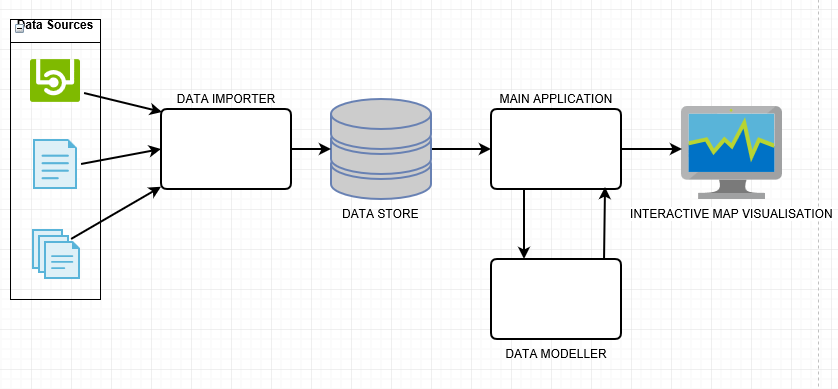
\includegraphics[scale=0.75]{figures/Software_Architecture} % Code example


%-----------------------------------
%	SUBSECTION 2
%-----------------------------------

\subsection{Architecture choices}
For this project two main technologies are being used, Python and Javascript. The majority of the software code has been written in Python, specifically for the data import processes, for the main application which runs the analysis and geocoding and the data modelling component. Python was chosen for these components for a number of factors. Firstly for the data importer, Python has excellent capabilities for data processing allowing the data to be collected and cleaned leveraging the Pandas module. For the main application, Python's geocoding and spatial capabilites were important factors in the choice. The ability to import shape files and reproject coordinate systems leveraging Geopandas and Shapely allowed more flexibility in which datasets were suitable for the project and the option to export to GeoJSON format facilitated the data visualisation.
For the visualisation stages Javascript embedded in a html file was chosen. For this final component of the project Javascript was preferred to Python due to the interactive element required on the map. With the aid of the Leaflet.js package in Javascript I was able to make use of more map features to present any end users with a more complete user experience.


%----------------------------------------------------------------------------------------
%	SECTION 2
%----------------------------------------------------------------------------------------

\section{Components}

The software architecture design for the project has been created with the aim of being able to isolate individual elements in the interest of performance. The system is not dependent on processing a live data feed so it is important that the component that imports the data does not have to run everytime a user would wish to access the interactive map visualisation. The design means that each component can be modified and without affecting the other parts.  


%-----------------------------------
%	SUBSECTION 1
%-----------------------------------
\subsection{Data inputs}
The data input layer is the base layer of the system. This consists of several different types of input including API feeds from the Foursquare platform, csv files collected directly from urls and other data files which have been pre-collected and loaded into the data store. This layer is the most likely to change moving forward as new and updated data sources are published or become available in alternative formats.

%-----------------------------------
%	SUBSECTION 2
%-----------------------------------

\subsection{Data importer}
The data importer software is written in Python and is designed as a series of functions. Each function imports one of the required datasets. Setting these up as seperate functions gives the option to run imports individually. This is an important requirement of the system as certain imports take a considerable amount of time. The iterative nature of the API imports combined with daily rate limits mean that it is only feasible to run the API imports from Foursquare on at most a daily basis. As the system is not reliant on a live feed, the data import software could be run as an overnight batch process. 

%-----------------------------------
%	SUBSECTION 3
%-----------------------------------

\subsection{Data store}
The data store is central to the architecture to safeguard performance levels. As the data imports are best suited to a batch process, the cleaned data files should be stored in the data store for the main application software to run efficiently. The data store is also used for any pre-collected data which cannot be collected directly from a url or API. This imports the data for the 18 base indicators which create the 6 well-being domains.

%-----------------------------------
%	SUBSECTION 4
%-----------------------------------

\subsection{Main application}
The main application software performs a variety of tasks and is written in Python. The first task that the software performs is to take the data that has been imported for the 18 base indicators from the data store. The main application then performs any data manipulation and applies a set of geocoding and spatial functions to standardise the data into a format where everything is aggregated for London Ward geometry. Having standardised, the software then creates the 6 well-being domains using functions drawing on Principal Component Analysis and mean calculation functions which also normalise the data to ensure that each score is between 0 and 100.
These 6 domains are then combined with data showing median house prices and the related quintiles and passed through the regression and classification models chosen through the data modeller component. The final task performed by this component is to create a geoJSON file including the well-being domain scores, median house price information, spatial data and predicted regression and classification values. This file contains the data used in the visualisation.

%-----------------------------------
%	SUBSECTION 5
%-----------------------------------

\subsection{Data modeller}


%-----------------------------------
%	SUBSECTION 5
%-----------------------------------

\subsection{Interactive map}
The final component of the software architecture is the interactive map which is built in javascript and html. This component builds a framework for the map using tiles from the MapBox service. A javascript function then takes the geoJSON file and add this as a layer to the map. This part of the architecture can be seen as the user front end as the visualisation allows users to hover over each ward to see the scores, actuals and predictions along with features such as a zoom facility.